\chapter{Assignment: Data Inspection}
\label{hw:data-inspection}

\newthought{Understanding the data is crucial} for any data science task. And the best way to achieve this is with visualizations. With the \widget{Datasets} widget load \textit{Employee Attrition} data set, which describes employees of a company with 32 features, such as age, job role, years at company, and so on. We also know, whether an employee resigned from the company (Attrition = Yes) or not (Attrition = No).

\begin{figure}[h]
  \centering
  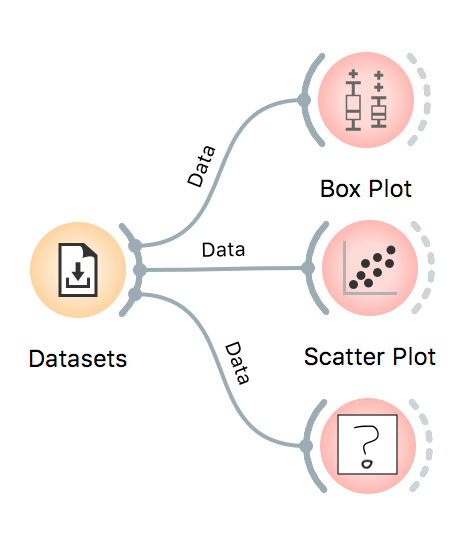
\includegraphics[scale=0.6]{workflow.png}%
  \caption{Workflow for the assignment.}
  \label{fig:data-inspection-workflow}
\end{figure}

Inspect the data to understand it better:
\begin{enumerate}
    \item Use \widget{Scatter Plot} and try \textit{Find Informative Projections}. How does the top combination look like? Is it useful? Why (not)?
    \item Use \widget{Box Plot} and try \textit{Order by relevance to subgroups}. Which attribute best splits the data by \textit{Attrition}? Explain it.
    \item Which widget would you use to observe relationship between two discrete variables in relation to Attrition? Use \textit{Find informative projections} in that widget and explore the top result.
\end{enumerate}